\section{Contexto y motivaci�n}

\subsection{Integraci�n Sem�ntica de los Recursos de Informaci�n en una Memoria Corporativa}
\begin{frame}
	\frametitle{Integraci�n Sem�ntica de los Recursos de Informaci�n en una Memoria Corporativa}
	\begin{block}{}
	\justifying
	\small B�squeda y recuperaci�n de informaci�n significativa existente en los recursos de informaci�n.
	\end{block}
	
	\begin{figure}
	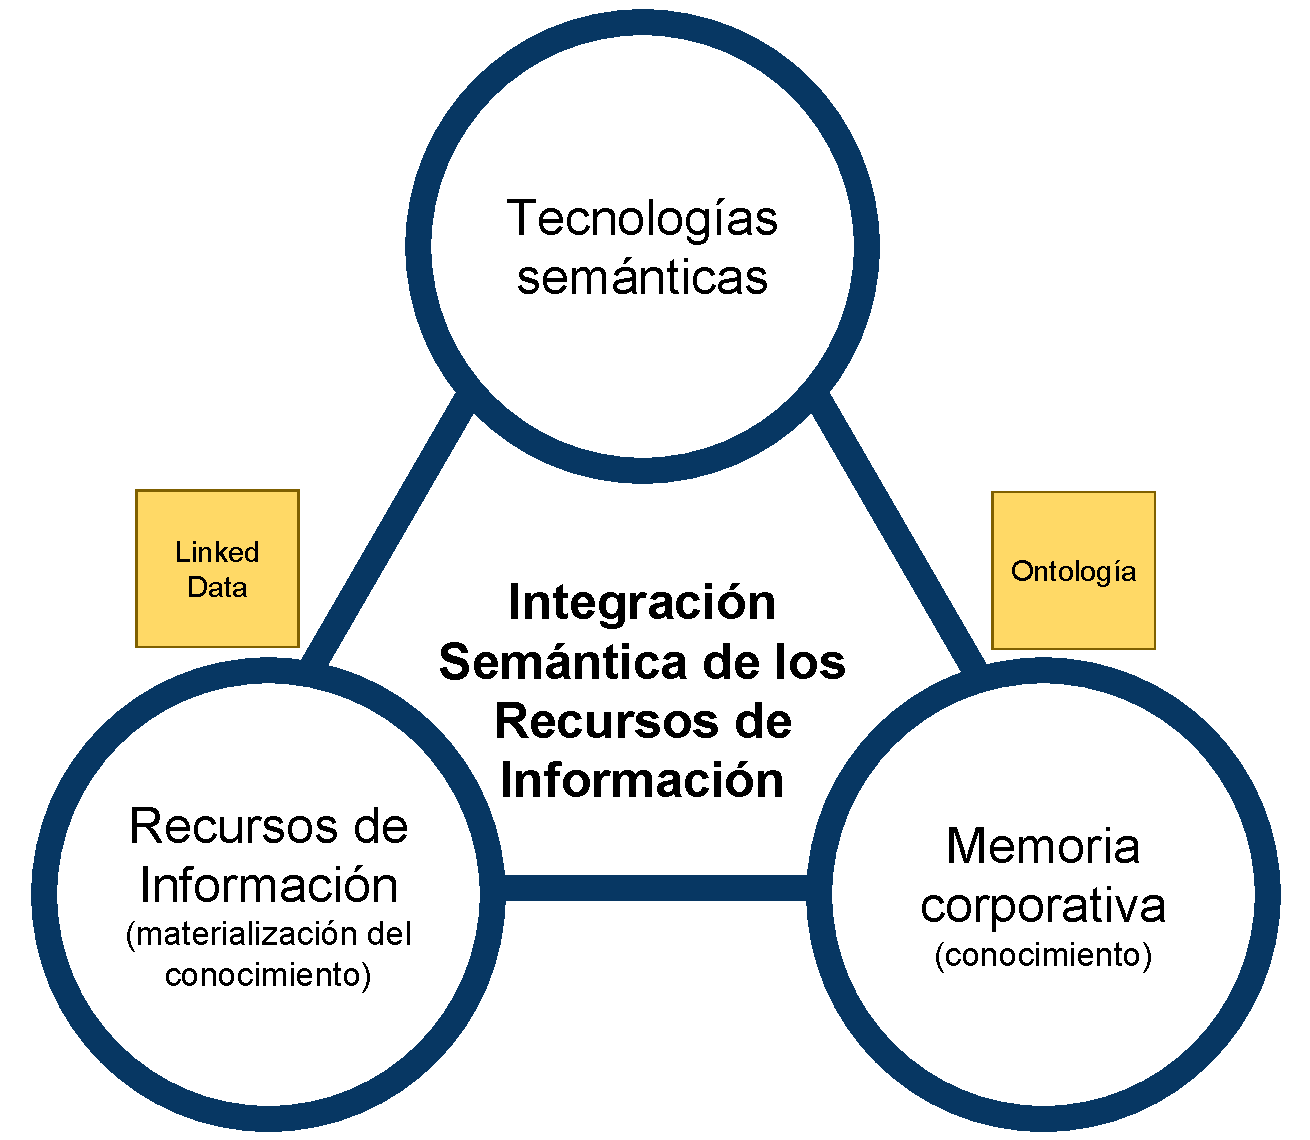
\includegraphics[scale=0.25]{ISRIMC} 
	\end{figure}
\end{frame}

\subsection{Memoria corporativa}
\begin{frame}
	\frametitle{Memoria Corporativa}
	%%%%%%%%%%%%%%%%%%%%%%%
	\begin{block}{Definici�n}
	\justifying 
	Una memoria corporativa (MC) es una representaci�n expl�cita, t�cita, consistente y persistente del conocimiento de una organizaci�n.
	\end{block}
	
	\begin{figure}[htbp]
	\centering
	\subfigure{
	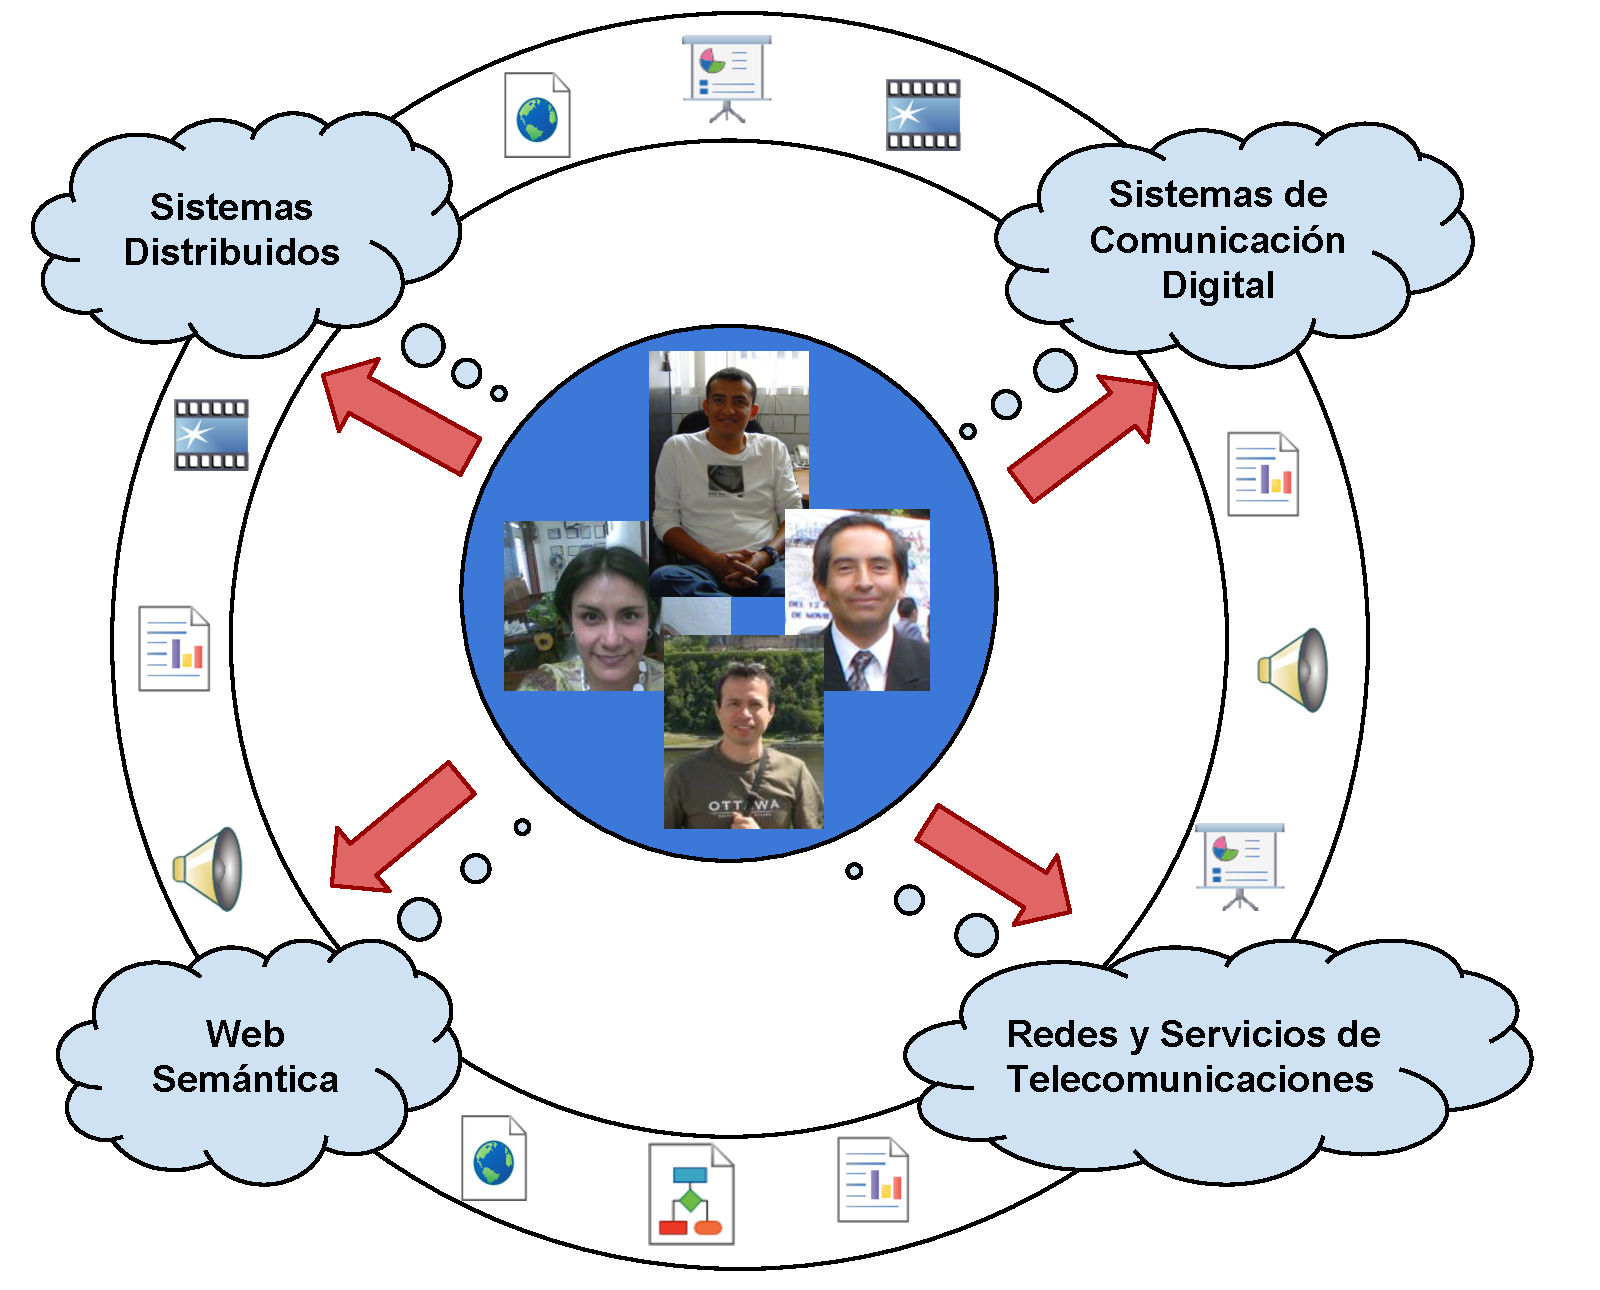
\includegraphics[scale=0.18]{ConocimientoRyT} 
	}
	\subfigure{
	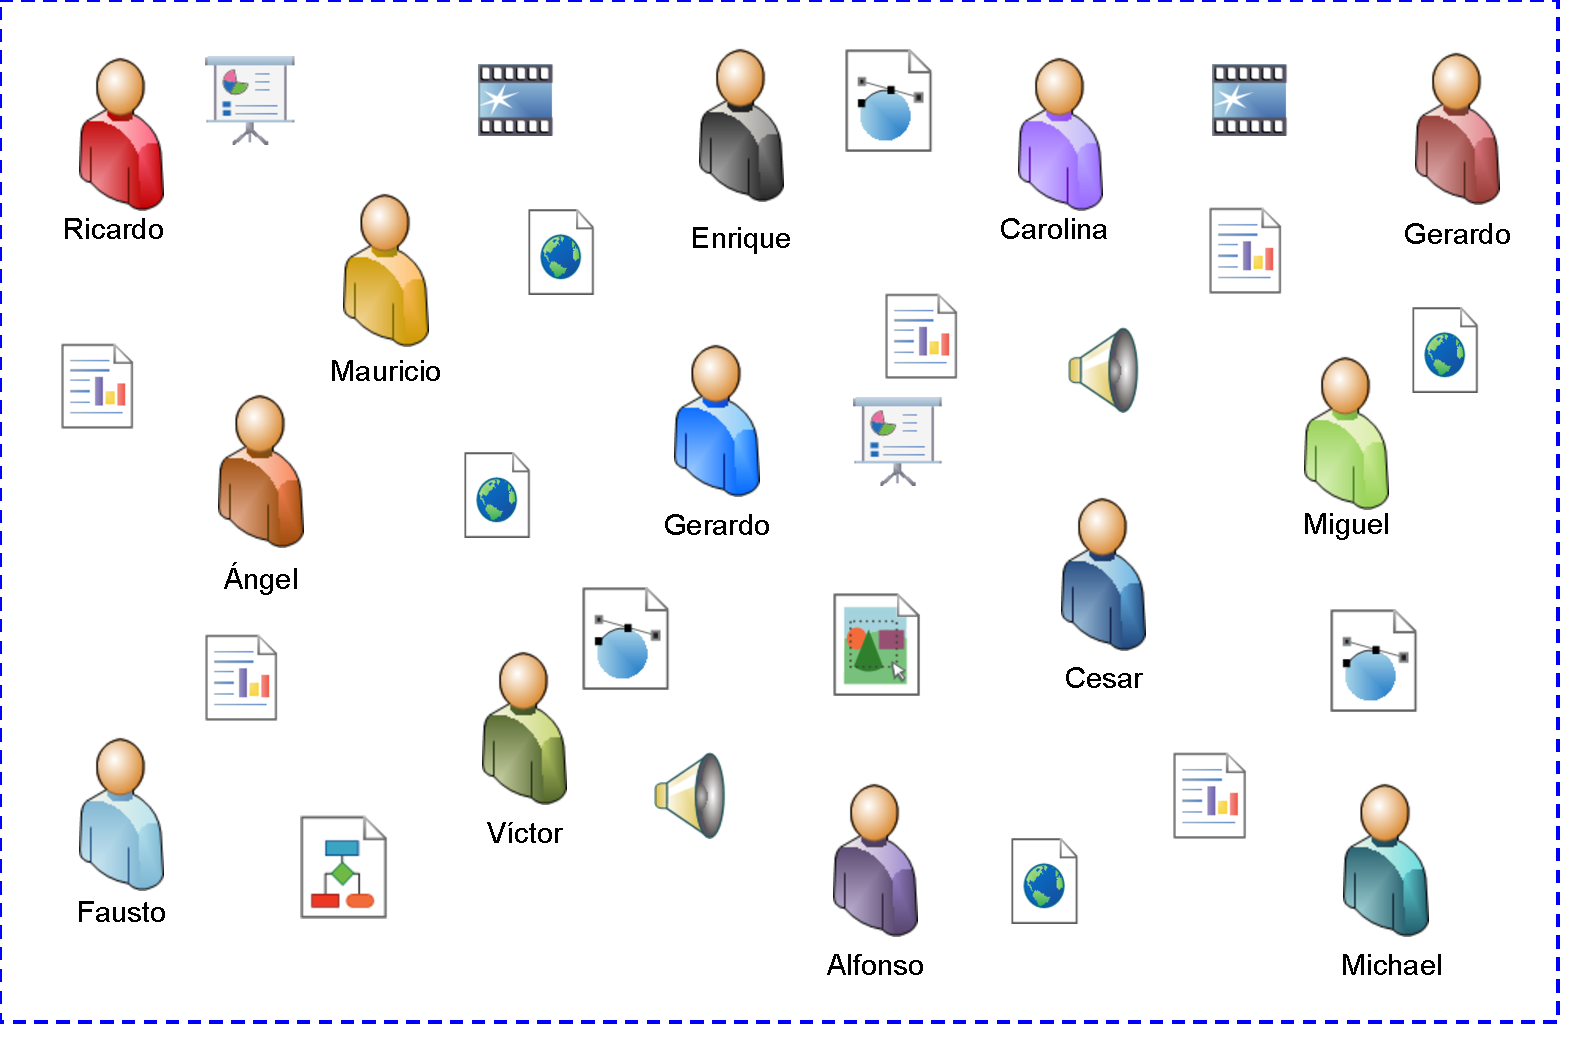
\includegraphics[scale=0.19]{EjemploMC} 
	}
	\end{figure}
	%%%%%%%%%%%%%%%%%%%%%%%
\end{frame}

\subsection{Recurso de Informaci�n}
\begin{frame}
	\frametitle{Heterogeneidad y significado de la informaci�n}
	\begin{figure}
	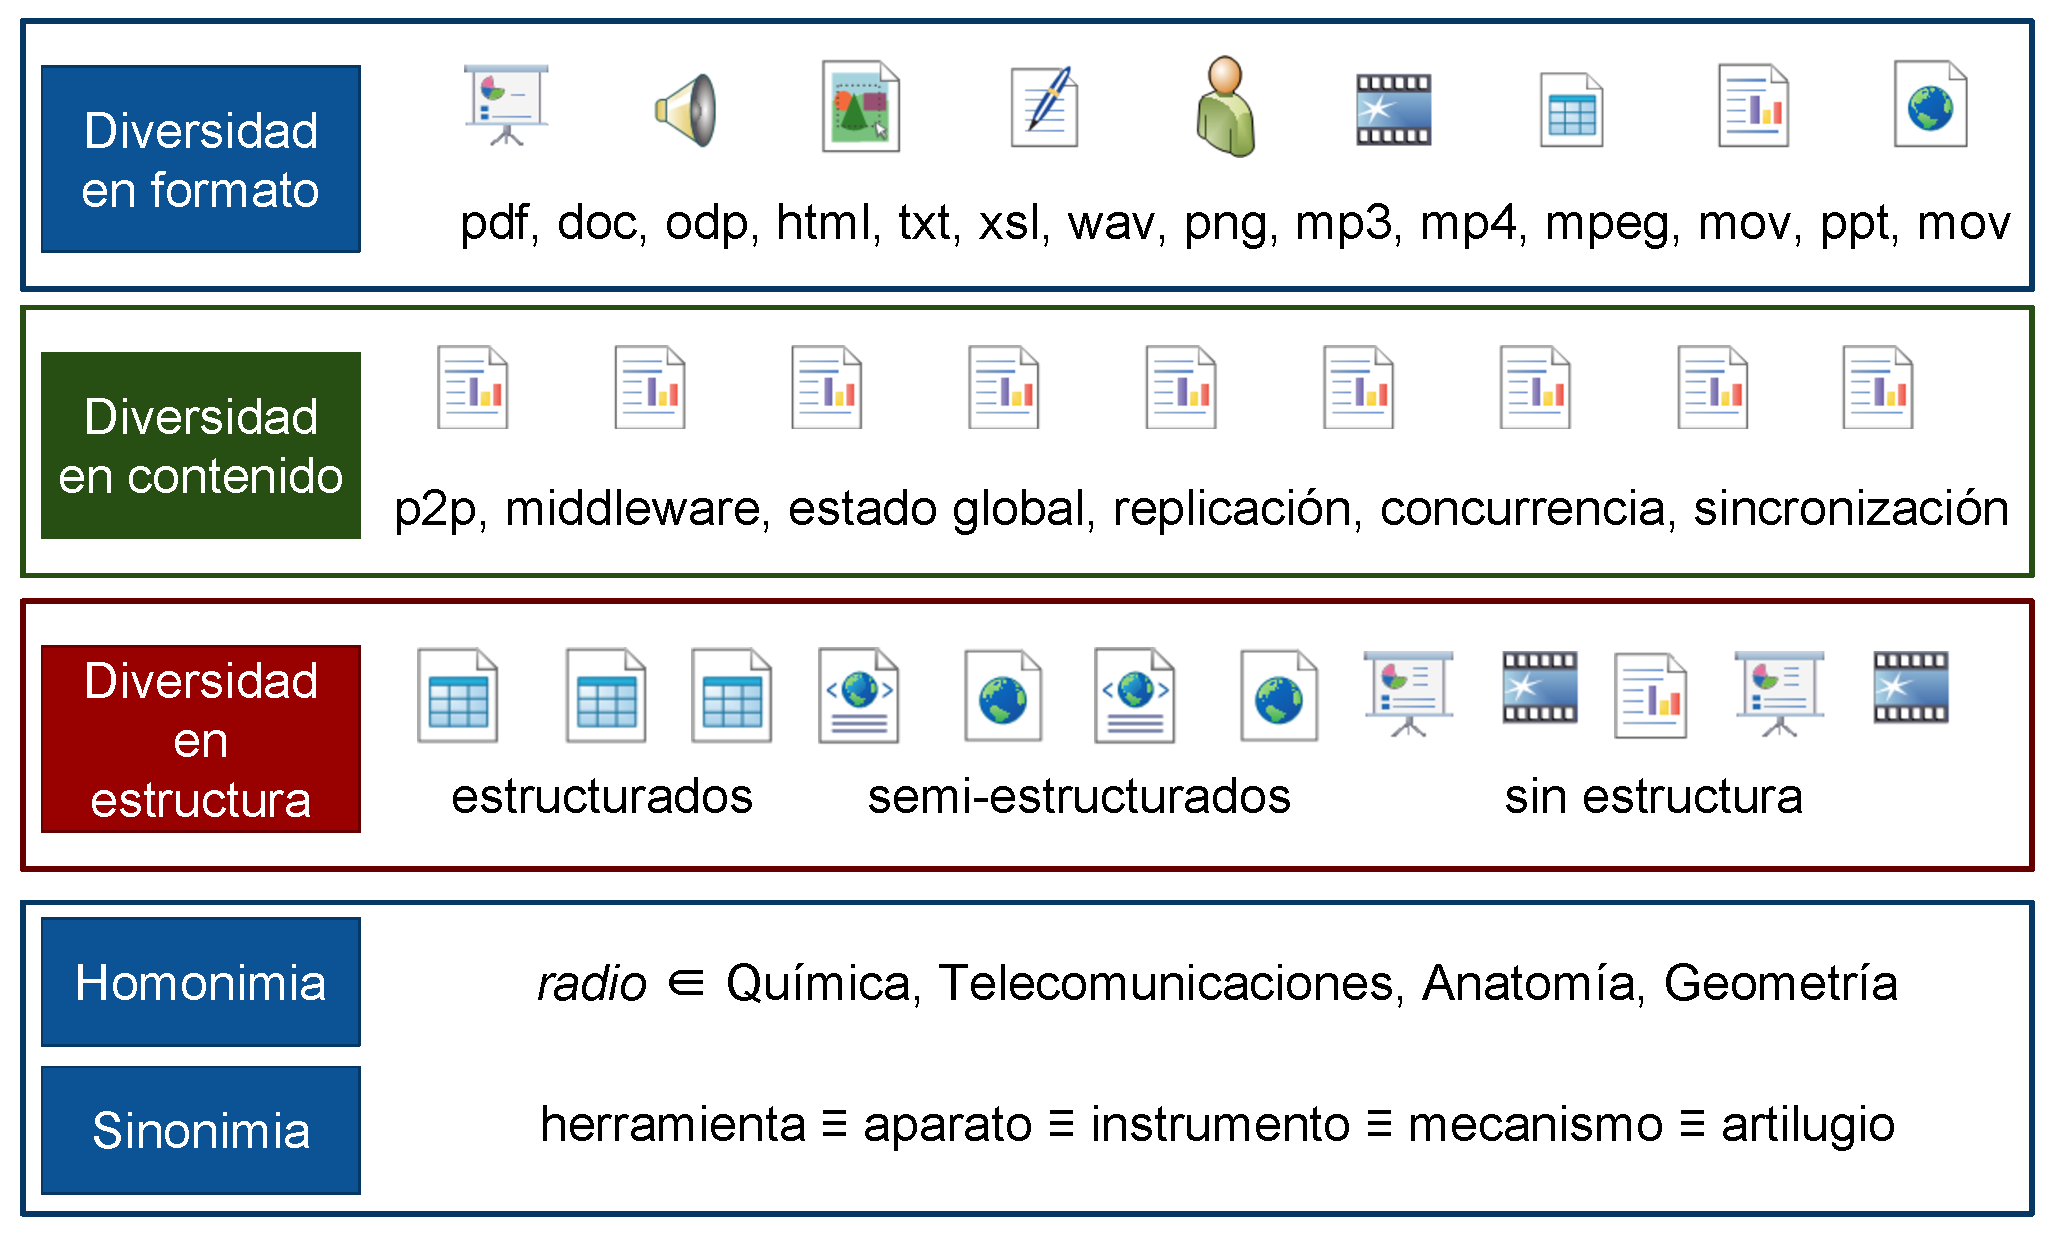
\includegraphics[scale=0.30]{NatMC} 
	\end{figure}
\end{frame}

\subsection{Tecnolog�as Sem�nticas}
\begin{frame}
	\frametitle{Tecnolog�as Sem�nticas}
	\begin{block}{Definici�n}
	\justifying 
	\small Las tecnolog�as sem�nticas (TS) son un conjunto de metodolog�as, lenguajes, aplicaciones, herramientas y est�ndares para suministrar u obtener el significado de las palabras, informaci�n y las relaciones entre �stos.
	\end{block}
	
	\begin{figure}
	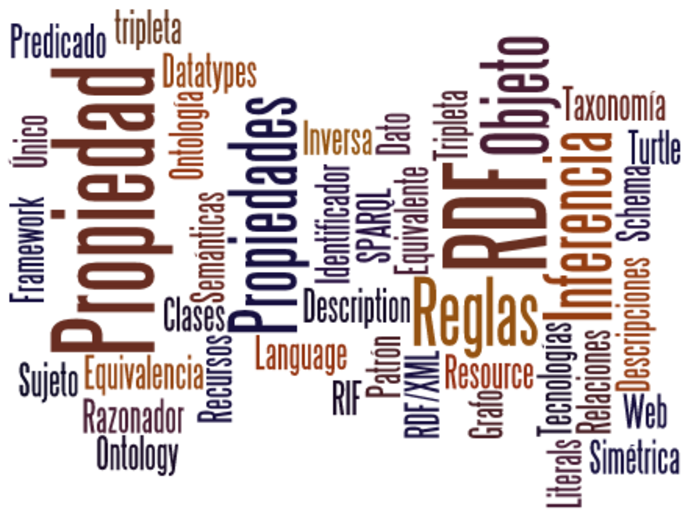
\includegraphics[scale=0.42]{TSWords} 
	\end{figure}
\end{frame}

\begin{frame}
	\frametitle{Integraci�n Sem�ntica de los Recursos de Informaci�n en una Memoria Corporativa}
	\begin{block}{Casos de Uso}
		\begin{itemize}%
		\item \justifying \textbf{\textit{Cartograf�a de Competencias}} es la b�squeda y recuperaci�n de informaci�n significativa de personas a partir de las caracter�sticas personales y profesionales de las mismas.
		\item \justifying \textbf{\textit{Recursos Digitales}} es la b�squeda y recuperaci�n de los documentos basados en texto y archivos multimedia a partir del contenido de los mismos.
		\end{itemize}
	\end{block}
	
	\begin{figure}
	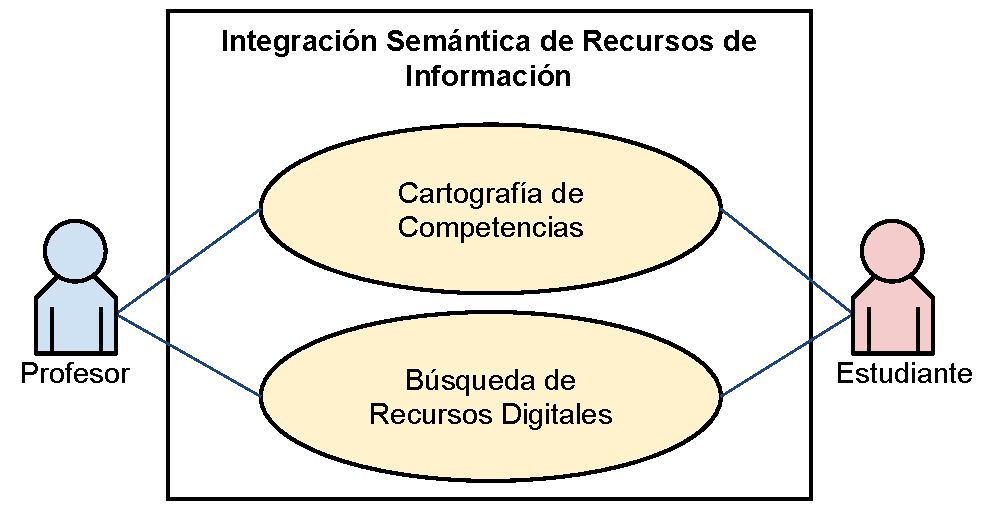
\includegraphics[scale=0.35]{CasosUso} 
	\end{figure}
\end{frame}

\subsection{Estado del Arte}
\begin{frame}
	\frametitle{Estado del Arte}
	\begin{block}{}
	\begin{enumerate}
	\item \justifying Representaci�n del conocimiento mediante el uso de tecnolog�as sem�nticas.
	\item \justifying B�squeda, recuperaci�n y/o publicaci�n de informaci�n usando modelos sem�nticos.
	\item \justifying Gesti�n sem�ntica de una memoria corporativa.
	\end{enumerate}
	\end{block}
	
	\begin{figure}
	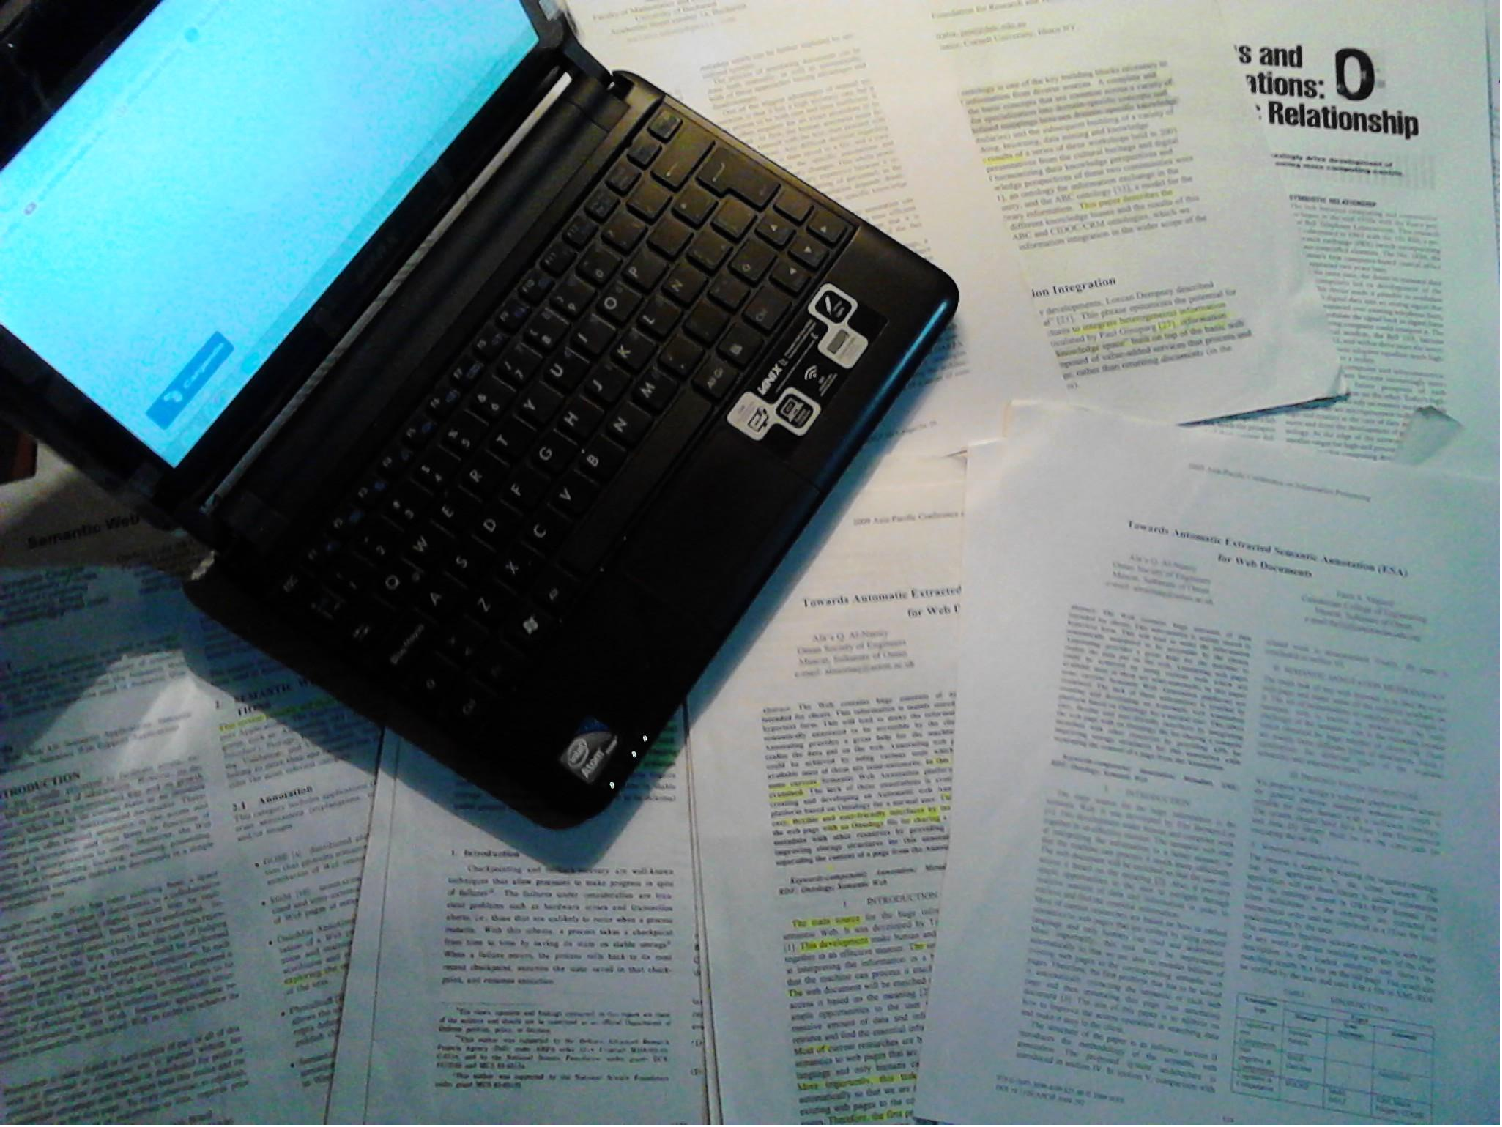
\includegraphics[scale=0.15]{EstadoArte} 
	\end{figure}
\end{frame}

\begin{frame}
	\frametitle{Comparativa}
	\begin{figure}
	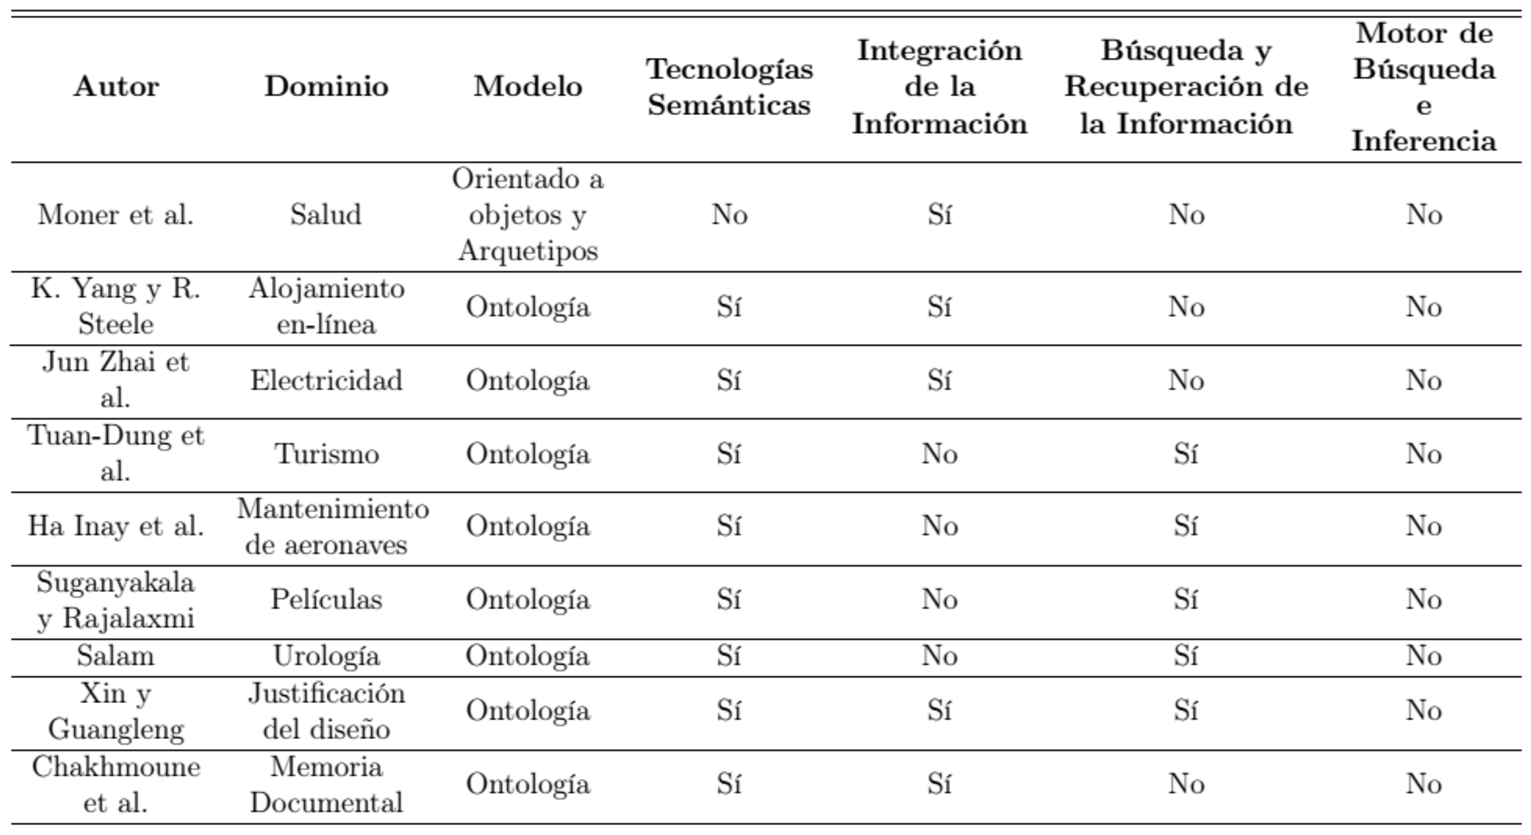
\includegraphics[scale=0.38]{TablaEOA} 
	\end{figure}
\end{frame}